\section{Cavity}
\frame{
\frametitle{Optical resonator}
\begin{itemize}
\item Fabry-Perot cavity
\end{itemize}
\begin{center}
\includegraphics[scale=0.4]{caivty_waves.pdf}
\end{center}

}

\frame{
\frametitle{Optical resonator}
\begin{itemize}
\item Cavity resonances
\end{itemize}
\begin{equation*}
\omega_n = 2\pi\cdot n\frac{c}{2L}
\end{equation*}
\begin{itemize}
\item Free spectral range
\end{itemize}
\begin{equation*}
\omega_{\mathrm{FSR}} = 2\pi\cdot\frac{c}{2L}
\end{equation*}
\begin{itemize}
\item Optical finesse
\end{itemize}
\begin{equation*}
\mathcal{F} = \frac{\omega_{FSR}}{\kappa}
\end{equation*}
\begin{itemize}
\item Loss rates
\end{itemize}
\begin{equation*}
\kappa = \kappa_{ex} + \kappa_{0}
\end{equation*}
}

\frame{
\frametitle{Cavity fields}
\begin{itemize}
\item Amplitude field analysis
\end{itemize}
\begin{center}
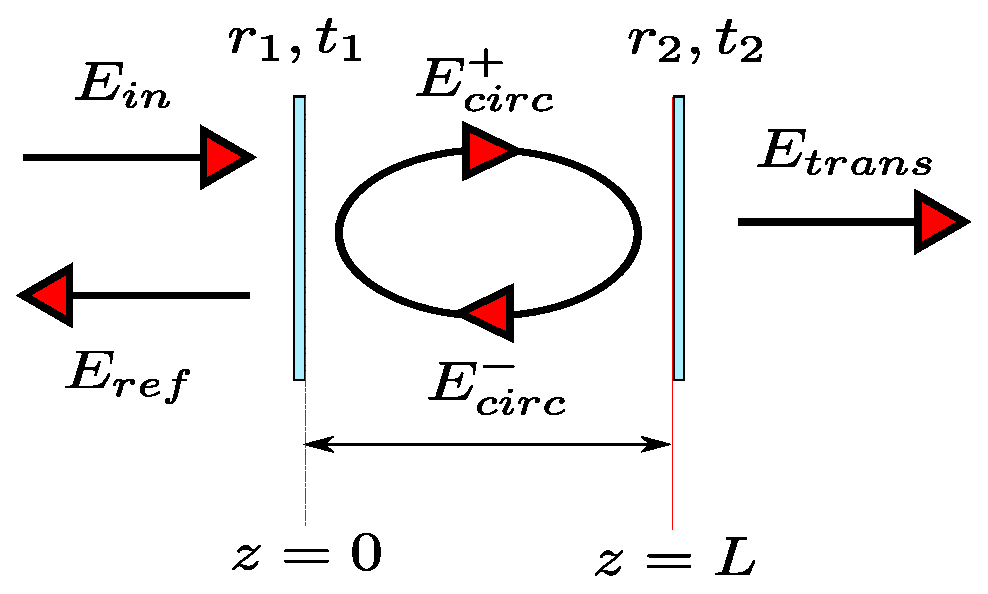
\includegraphics[scale=0.4]{E-field_model_edit.eps}
\end{center}
}

\frame{
\frametitle{Cavity steady state}
\begin{itemize}
\item Steady state solution
\end{itemize}
\begin{center}
\includegraphics[scale=0.45]{cavity_model_fsr.pdf}
\end{center}
}

\frame{
\frametitle{Cavity EOM}
\begin{itemize}
\item Rescaled intra-cavity field $E_{circ}(t)\sqrt{T_{rt}} = a(t)$
\item Cavity equation of motion
\end{itemize}
\begin{equation*}
\dot{a}(t) = -\left(\frac{\kappa}{2} + i\Delta\right)a(t) + \sqrt{\kappa_1}E_{in}(t)
\end{equation*}
\begin{itemize}
\item Circulating power
\end{itemize}
\begin{equation*}
\langle P_{circ} \rangle = \frac{\mathcal{F}\kappa}{2\pi\kappa_2}\langle P_{trans} \rangle
\end{equation*}
}

\section{Optomechanics}
\frame{
\frametitle{Optomechanics}
\begin{itemize}
\item Cavity with moving boundary
\item Mechanical degree of freedom
\item Frequency shift per displacement $G$
\end{itemize}
\begin{center}
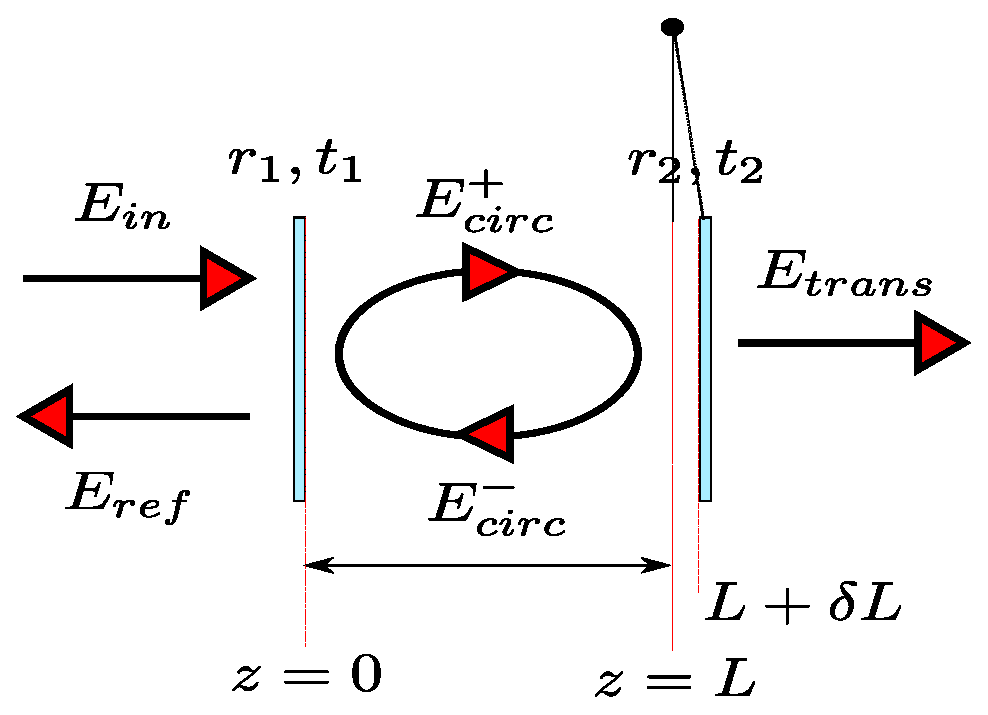
\includegraphics[scale=0.45]{E-field_model.eps}
\end{center}
}

\frame{
\frametitle{Coupling}
\begin{itemize}
\item Photon momentum transfer onto mirror
\end{itemize}
\begin{equation*}
\Delta p = \frac{2h}{\lambda}
\end{equation*}
\begin{itemize}
\item Radiation pressure force
\end{itemize}
\begin{equation*}
F_{rad} = -G\frac{U_{circ}}{\omega_c}
\end{equation*}
\begin{itemize}
\item Coupled equations of motion
\end{itemize}
\begin{equation*}
\dot{a}(t) = -\left( + \frac{\kappa}{2} + i(\Delta - Gx(t)) \right)a(t) + \sqrt{\kappa_1}E_{in}
\end{equation*}
\begin{equation*}
\frac{1}{m}\left( F_{th}(t) + F_{rad} \right) =\ddot{x}(t) + \Gamma_m\dot{x}(t) + \Omega_m^2\delta x(t)
\end{equation*}
}

\frame{
\frametitle{Linearization}
\begin{itemize}
\item Linearized equation of motion $a(t) =  \langle a \rangle + \delta a(t)$
\end{itemize}
\begin{equation*}
\delta \dot{a}(t) = -\left(\frac{\kappa}{2} + i\bar{\Delta}\right)\delta a(t) - iG\delta x(t)\langle a \rangle
\end{equation*}
\begin{equation*}
\frac{1}{m}\left( \delta F_{th}(t) + \delta F_{rad}(t) \right) = \delta \ddot{x}(t) + \Gamma_m\delta\dot{x}(t) + \Omega_m^2x(t)
\end{equation*}
}

\frame{
\frametitle{Optical induced effects}
\begin{itemize}
\item Optical spring effect $\Delta\Omega_{opt}$
\item Optical induced damping $\Gamma_{opt}$
\end{itemize}
}

\frame{
\frametitle{Cavity enhanced effects}
\begin{itemize}
\item Resolved sideband regime $\kappa \ll \Omega_m$
\end{itemize}
\begin{center}
\includegraphics[scale=0.5]{resolved_sb.pdf}
\end{center}
}